The goal was to estimate the maximum possible jump height of a joint torque driven model.
Only the impulsion phase is simulated.
The impulsion is divided in two phases, first phase with 2 contacts (heel and toe),
and second phase with 1 contact (only toe). Each phase time was constrained to a minimum and a maximum:

\begin{tabular}{c c c}
& Phase & Min & Max \\
\hline
$\#1$ & $0.2$s & $1.0$s \\
\hline
$\#2$ & $0.05$s & $1.0$s \\
\end{tabular}

The actuators are modeled using a custom constraint which computes the torque range from q and qdot. This is done
using the gauss3p function of biorbd using predetermined factors. (\ref{fig:graph_force_vitesse_longueur})

The first term of the objective function corresponds to the jump height. The weight is negative to maximize the height
instead of minimizing it. The second term of the objective function corresponds to the time variation. It allows the
solver to get the best jump with the shortest time.

The problem was solved using ipopt.
The problem is first launched using the BFGS hessian approximation feature for 200 iterations. Then
if the maximum number of iteration is reached, the solution is re-optimized for 1000 iterations using a warm start 
with the results.

\begin{figure*}[t!]
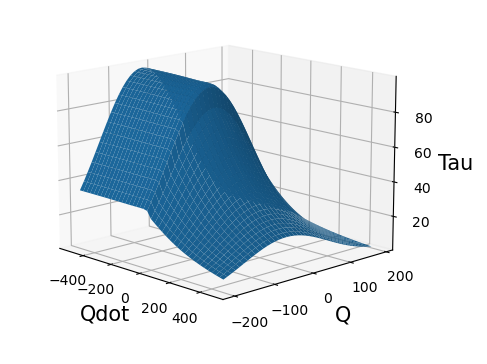
\includegraphics[width=\textwidth/2]{figures/graph_force_vitesse_longueur.png}\\
\caption{Surface getting torque range from q and qdot}
\label{fig:graph_force_vitesse_longueur}
\end{figure*}
